\documentclass[relqm.tex]{subfiles}

\begin{document}
\part{Particle Physics Phenomenology}
\chapter{A Brief History...}
The modern outlook of particle physics is based on these elementary particles:
\textit{draw table of all particles}
Back in the 1940s, we did not have the same scope. 
We knew about protons, neutrons, and electrons. 
Then we discovered pions and muons coming in from the atmosphere, using cloud chambers and their difference of decay rate to distinguish them.
So we added the muon to our elementary particles.
Pions hinted towards the existence of quarks, made of u and d quarks.

\section{...of QCD}
\begin{itemize}
    \item Not long after, we discovered the Kaon as well. 
        We saw something decay into two pions which had to be heavier. 
        Kaons contain the s quark, so lead eventually to the higher generations of quarks. 
    \item Over time, more particles were slowly discovered, e.g. myriads of mesons like $\pi$, K, $\rho$, $\eta$, etc. 
    \item Gell-Mann realised that all these particles we were finding could be made up of more elementary particles called quarks, with different combinations and numbers yielding the different particles we knew at this time.
        There was no evidence at this time that this would be the case, it was just a useful thought experiment. 
    \item In the late 60s, the Stanford accelerator used deep inelastic scattering to decompose the proton and resolve its constituents, i.e. the parton model leading to confirmation of quarks.
    \item Gell-Mann and others fledge out their theory of quarks into a full gauge theory into what we know today as SU(3) QCD.
        This was ultimately confirmed when the $J/\Psi$ ($c\bar{c}$) was discovered by two separate accelerators, so now the quark model for the first two generations was found and made sense of the current catalogue of composite particles.
    \item Shortly after, we found experimental confirmation of the gluon, making sense of quarks as a gauge theory. 
    \item We then discovered the $\Upsilon$ ($b\bar{b}$) meson in the mid 70s, which hinted at a third generation of quarks, but the top quark was to remain elusive until \~95.
\end{itemize}

\section{...of GSW Theory}
\begin{itemize}
    \item In the mid 50s, we found interactions between protons and neutrinos to form neutrons and leptons, both for first and second generation.
    \item We required the same number of generations of quarks and leptons, and slowly we found the third generation of leptons by 2000 with the discovery of $\nu_\tau$.
    \item The interactions with neutrinos studied hinted to some other interaction besides electromagnetism and QCD, with its strength described in the Fermi constant. 
        These interactions all seemed pointlike to us as the particle mediating them was so much heavier than the others. 
    \item Glashow et al formed this into a gauge theory to attempt to describe this, finding the $W^\pm,Z$ bosons, as well as combining this with the electromagntic gauge theory to form the electroweak of SU(2)$\times$U(1).
    \item In the 1980s at CERN, electrons and positrons were collided to produce the $W^\pm,Z$ bosons and measured their masses as \~80 and 90 GeV respectively, values which were predicted back in the 60s by Weinberg and Salam.
\end{itemize}

\section{...of the Higgs theory}
\begin{itemize}
    \item The big issue we had was that all our theories worked on gauge invariance which would be broken by mass terms to form the masses we knew these particles had. 
    \item Many people postulated what we now know as the Higgs mechanism at roughly the same time, in the 60s. 
    \item Very skeptical for many years about this theory, although it was seen as the simplest way to get it done. 
        Then in 2012, CERN found what we believe to be the Higgs boson, completing the current picture of particle physics, encompassing all forces, interactions, and particles predicted by the Standard Model.
\end{itemize}

\section{Some Notes on Notation and Terminology}
\begin{itemize}
    \item Pions, Kaons, and any other particles made of one quark and an anti-quark are known as \textbf{Mesons}.
    \item Neutrons, protons, and other three-quark particles are known as \textbf{Baryons}.
    \item Overall, any particle made of quarks is called a \textbf{Hadron}.
    \item Leptons never really form bound states until electrons are bound by atoms, so there is not much terminology for them. 
\end{itemize}
Next time, we will discuss particle colliders and their two parameters, COM energy and Luminosity. 
Collider physics is governed by the rate of events,
\begin{equation}
    \frac{dN_{ev}}{dt} = L\sigma,
\end{equation}
where $L$ is luminosity and $\sigma$ is the cross-section.

\chapter{The LHC}
Collisions between two particles are the basis for experimental particle physics. 
Particles have four -momenta $p=(E_p,\vp)$, where the total four-momenta going in will be $p_T=(E_1+E_2,\vp_1+\vp_2)$.
We can transform between coordinate systems of our four-momenta as
\begin{align}
    \frac{1}{\sqrt{1-v^2}}\begin{pmatrix}1& -\vv \\ -\vv & 1\end{pmatrix}\begin{pmatrix} E_1 \\ \vp_1\end{pmatrix} &= \frac{1}{\sqrt{1-v^2}}\begin{pmatrix} E_1-\vv\vp_1 \\ -\vv E_1 - p_1\end{pmatrix} \\
                                          &= \tensor{\Lambda}{_\mu^\nu}p_\nu
\end{align}
We can choose the simplest frame for this, i.e. the COM frame:
\begin{align}
    (p_1+p_2)_{cm} &= \begin{pmatrix} E_1^{cm} + E_2^{cm} \\ 0 \end{pmatrix} \\
    \frac{1}{\sqrt{1-v^2}}\begin{pmatrix}1& -\vv^{cm} \\ -\vv^{cm} & 1\end{pmatrix}\begin{pmatrix} E_1 + E_2 \\ \vp_1 + \vp_2\end{pmatrix} &= \frac{1}{\sqrt{1-v^2}}\begin{pmatrix} E_1 + E_2 -\vv^{cm}(\vp_1+\vp_2) \\ -\vv^{cm}( E_1+E_2) - \vp_1-\vp_2\end{pmatrix}  \\
    s = (E_1^{cm}+E_2^{cm})^2 &= (p_1+p_2)^\mu(p_1+p_2)_\mu = (E_1+E_2)^2 - (\vp_1+\vp_2)^2
\end{align}
The LHC currently has a COM energy of 13 TeV, i.e. during proton-proton collisions, each proton as $E_p=6.5\,$TeV, with three-momenta equal in magnitude with opposite signs. 
Consider proton at rest ($p_1=(m_p,0)$) colliding with electron ($p_2=(E_2,\vp_2)$):
\begin{align}
    s = (p_1+p_2)^2 &= (m_p+E_2)^2 = m_p^2 + 2E_2m_p + \underbrace{E_2^2-p_2^2}_{m_e^2} \\
    E_{cm} = \sqrt{s} &= 100\,\text{GeV}
\end{align}
So we switched from fixed targets to two moving targets as it massively increases COM energy available, although we will see that not all this energy is the energy available for particle production. 
We consider the cross-section concept for proton collisions, where
\begin{align}
    \frac{dN_{ev}}{dt} &= 2vn_2N_1\sigma = L\times\sigma,
\end{align}
so the number of events occuring is dependent on the cross-section of the beams.
We have defined $L$ as the instantaneous \emph{luminosity}, which is like flux in astronomy etc. 
So the number of events is dependent on the cross-section of beam collisions and the how often particles are included within the cross-section (in the Luminosity).
We can describe each of the particles in these collisions using a Gaussian profile density of form
\begin{align}
    \rho &= \exp\left(-\frac{x^2}{2\,dx^2}-\frac{y^2}{2\,dy^2}-\frac{z^2}{2\,dz^2}\right).
\end{align}
We can then write the Luminosity as
\begin{align}
    L &= \frac{fN_1N_2N_b}{4\pi\,dx\,dy}.
\end{align}
We do not have a continuous beam of particles in these colliders, but a small collection of beams, where there will be $N_b$ travelling in each direction.
The Luminosity of the LHC is $L_{int}=140\,\text{fb}^{-1}$, where fb is defined as femtobarn ($1\,$fb $=10^{-15}\,$b $=10^{-39}\,$cm$^2$).
If we consider the cross-section of proton collisions for Higgs production, $\sigma_{pp\to h}=4\times10^4\,$fb, we can calculate the number of Higgs produced at the LHC as $N_{h}=5.6\times10^6$.

\section{The CMS detector at CERN}
\begin{figure}[H]
    \centering
    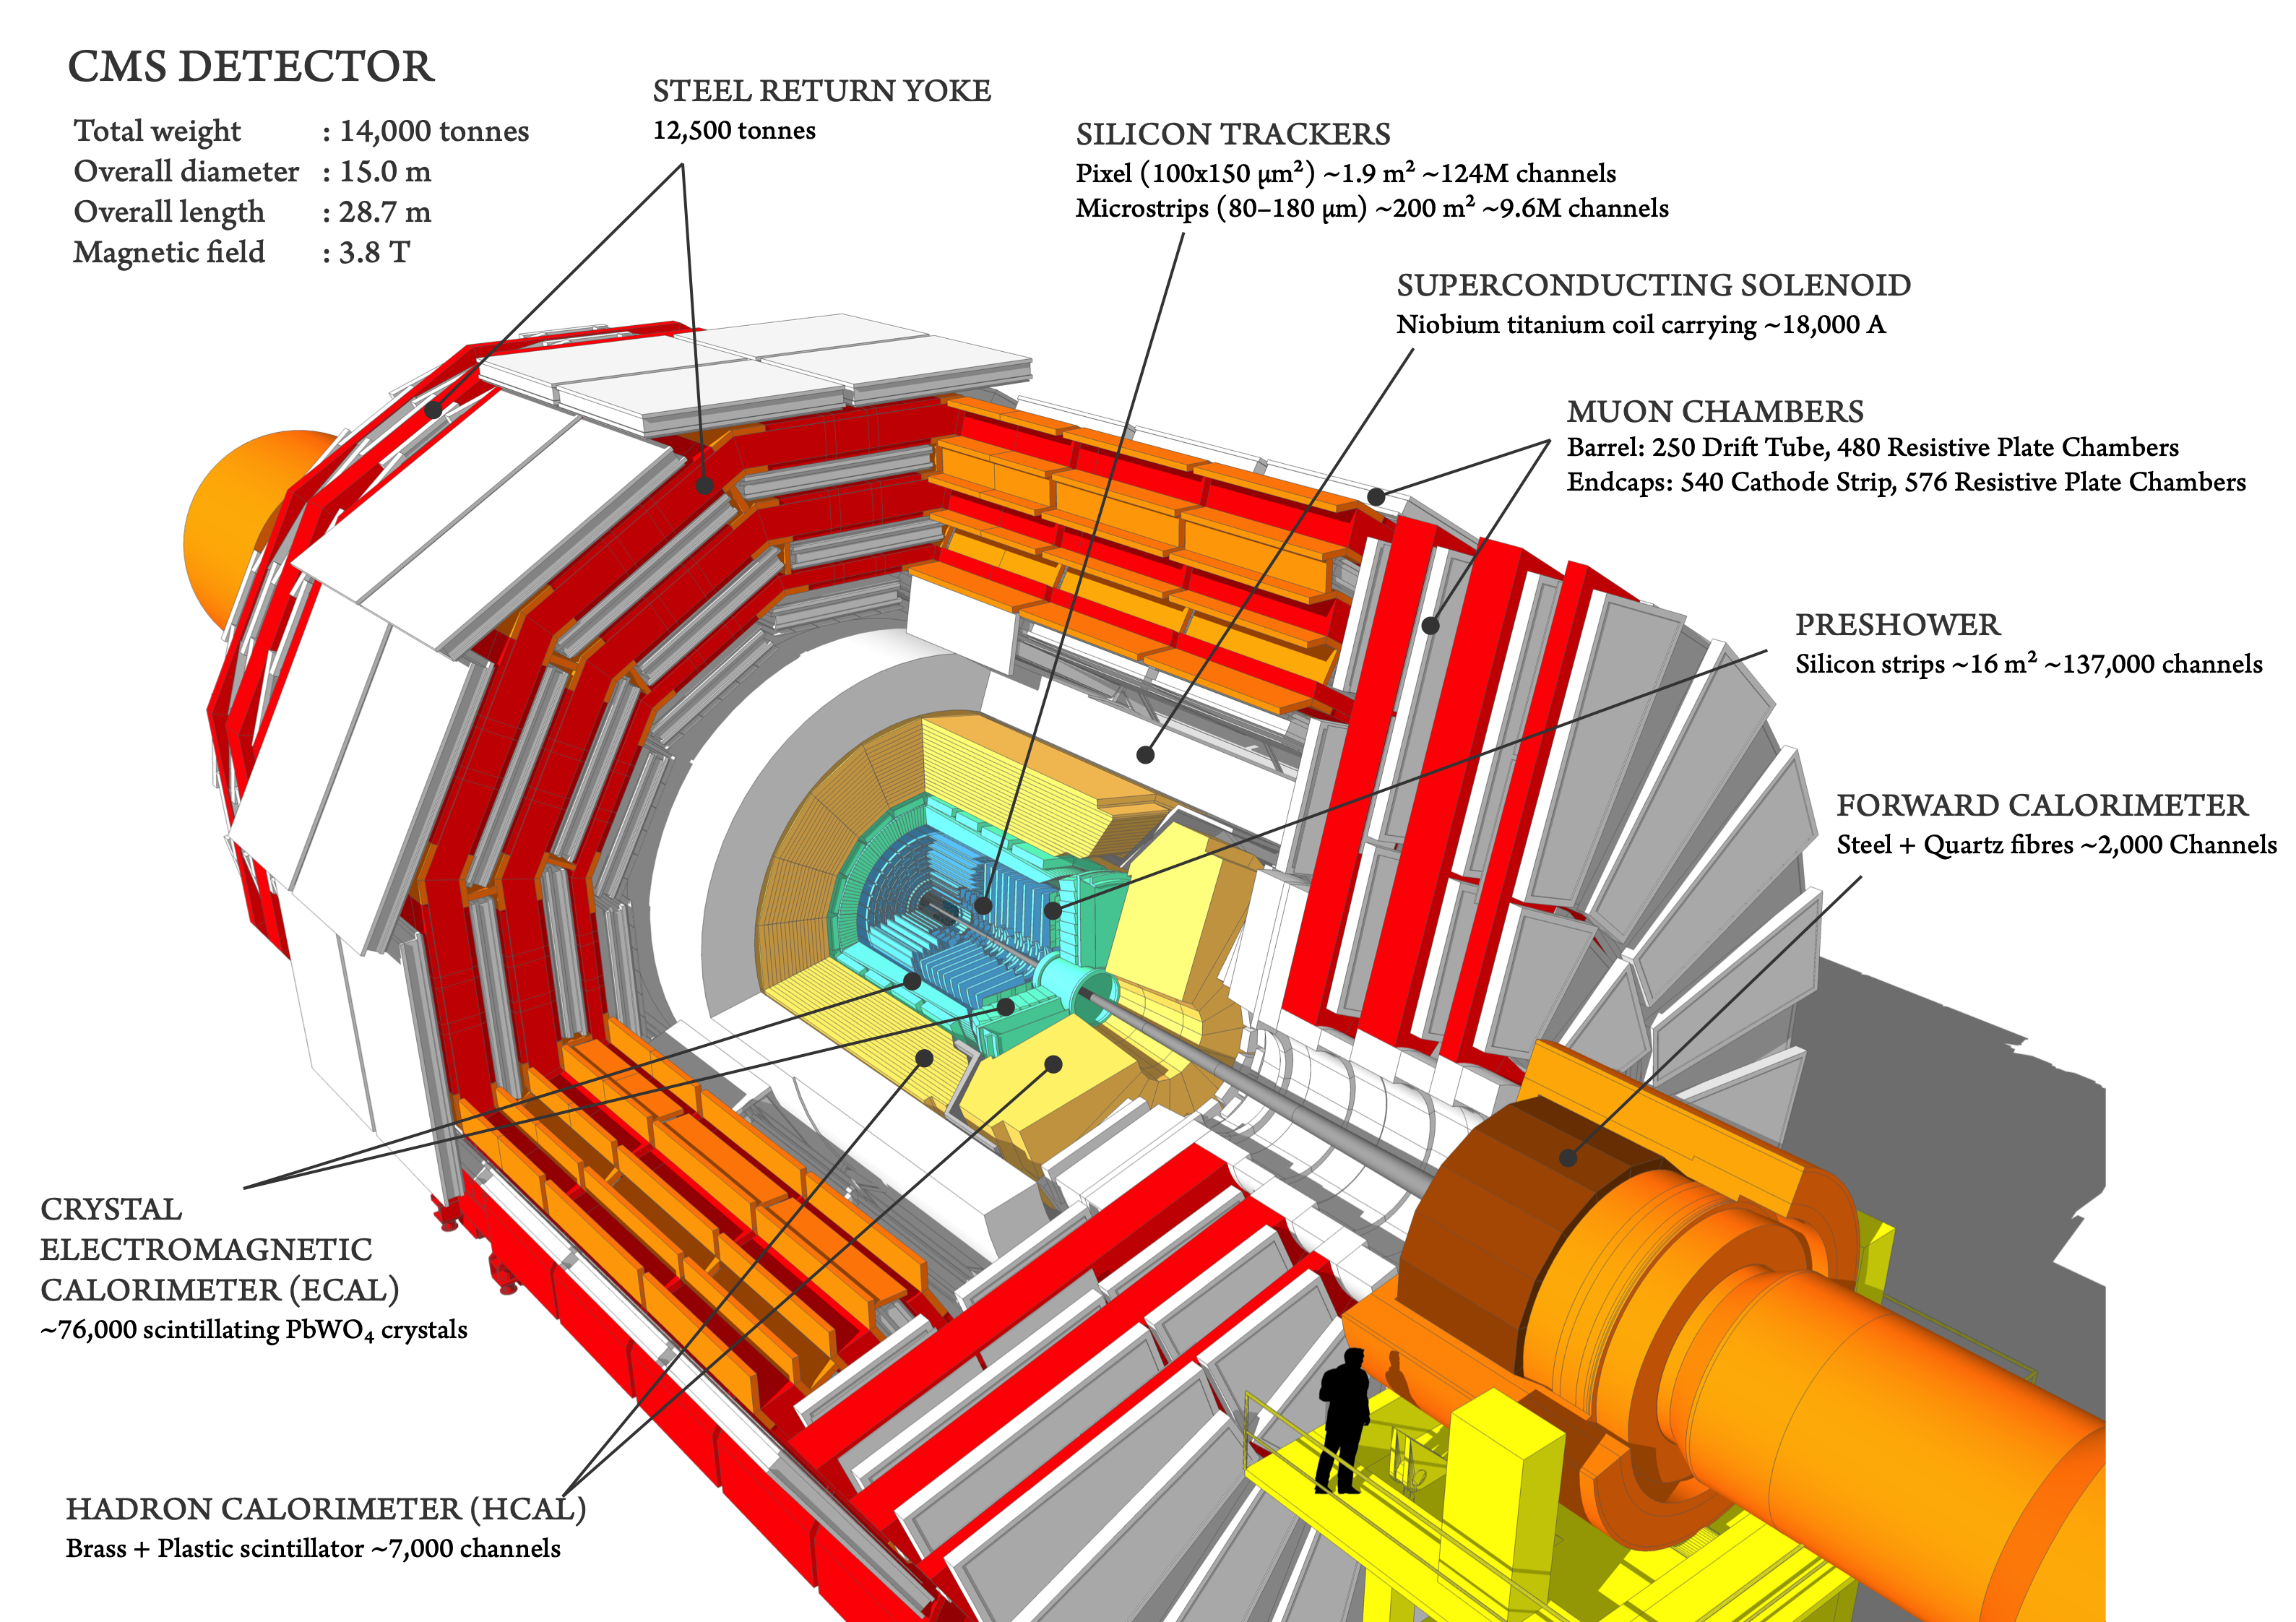
\includegraphics[width=0.9\textwidth]{CMS_160312_06.png}
\end{figure}
\begin{itemize}
    \item CMS (Compact Muon Solenoid) is a 14000 ton experiment, $15\times15$m$^2$.
    \item We have a ``tracker" made out of silicon which tracks the particles, as charged particles' paths are bent moving through it due to the magnetic field generated by the surrounding superconductor.
    \item The particles will then collide into a ``electromagnetic calorimeter" which allows us to measure their energy if they are electrons. 
    \item There is then a ``hadron calorimeter" which will collide with hadrons, i.e. pions, and measure their energy. 
    \item Finally there is a muon chamber, which of course detects muons.
    \item Neutrinos will not be detected by any of these chambers, but we can infer if one has been produced through the starting energy/masses and the measured outputs of electrons, hadrons, and muons. 
        Other low-interacting particles could be present in this as well, but so far all scattering events observed have been consistent with the missing particles being neutrinos.
\end{itemize}
We write length in units of $\frac{1}{\text{GeV}}$, which makes sense, when you multiply by $\hbar c$ and propagate through, it is then in units of approximately $2\times10^{-16}$m.
This length scale will explain why we do not observe quarks on their own - they hadronise in a shorter time than it takes for us to observe them. 
Top quarks can however be observed on their own as their lifetime is shorted than the hadronisation time due to their significant mass, $m_t=172.9\,$GeV.

\chapter{Path Integrals and Feynman Rules}
Consider a quantum system with our conjugate operators $\hat{Q}$ and $\hat{P}$. 
These satisfy the familiar defintions:
\begin{align}
    [\hat{Q},\hat{P}] &= i\hbar & \hat{Q}|Q\rangle &= Q|Q\rangle \\
    \langle Q|P|\rangle &= e^{iQP/\hbar} & \hat{P}|P\rangle &= P|P\rangle.
\end{align}
We can now consider the time evolution of the system using the time-dependent Schrodinger equation,
\begin{align}
    i\hbar\dpt|Q(t)\rangle &= \Ham, & \Ham &= \frac{\hat{P}^2}{2} + V(\hat{Q}).
\end{align}
We consider a non-relativistic object moving in one dimension with unit mass $M=1$.
The amplitude is therefore
\begin{align}
    \langle Q_F|e^{-i\Ham T/\hbar}|Q_I\rangle.
\end{align}
We break the time $T$ into $N+1$ intervals, such that $\delta t = T/(N+1)$, and evaluate the operators in terms of eigenvalues using several identities. 
\begin{align}
    \langle Q_F|e^{-i\Ham T/\hbar}|Q_I\rangle &= \langle Q_F|e^{-i\Ham \delta t/\hbar}\dots e^{-i\Ham \delta/\hbar}|Q_I\rangle \\
                                              &= \int \langle Q_F|e^{-i\Ham \delta t/\hbar}|Q_{N-1}\rangle\dots\langle Q_2|e^{-i\Ham\delta t/\hbar}|Q_1\rangle\langle Q_1|e^{-i\Ham\delta t/\hbar}|Q_I\rangle\prod_i dQ_i.
\end{align}
We can break down each product of this:
\begin{align}
    \langle Q_{j+1}|e^{-i\Ham\delta t/\hbar}|Q_j\rangle &= \int \langle Q_{j+1}|e^{-i\Ham\delta t/\hbar}|P\rangle\langle P|Q_j\rangle\frac{dP}{2\pi} \\
                                                        &= \int \langle Q_{j+1}|P\rangle e^{-i\frac{\delta t}{\hbar}(\frac{P^2}{2}+V(i\hbar\frac{\p}{\p P}))}\langle P|Q_j\rangle\frac{dP}{2\pi} \\
    &= \int e^{i\frac{Q_{j+1}P}{\hbar}}e^{-i\frac{\delta t}{\hbar}(\frac{P^2}{2}+V(i\hbar\frac{\p}{\p P}))}e^{-i\frac{Q_jP}{\hbar}}\frac{dP}{2\pi}.
\end{align}
The argument of the exponential is then:
\begin{align}
    -\frac{i\delta t}{\hbar}\left(\frac{P^2}{2}-\frac{P}{\delta t}(Q_{j+1}-Q_j)+V(Q_j)\right) &= -\frac{i\delta t}{\hbar}\left(\frac12\left(P - \frac{Q_{j+1}-Q_j}{\delta t}\right)^2 - \frac{(Q_{j+1}-Q_j)^2}{2\delta t^2} + V(Q_j)\right).
\end{align}
We can see that the integral in P is Gaussian which in general yields
\begin{align}
    \ifnt \exp\left(-\frac{(z-b)^2}{2a^2}\right)\,dz &= \sqrt{2\pi a^2},
\end{align}
so therefore the integral in P is
\begin{align}
    \int \langle Q_{j+1}|e^{-i\frac{\Ham\delta t}{\hbar}}|P\rangle\langle P|Q_j\rangle\frac{dP}{2\pi} &= \sqrt{\frac{\hbar}{i2\pi\delta t}}\exp\left[\frac{i\delta t}{\hbar}\left(\frac{(Q_{j+1}-Q_j)^2}{2\delta t^2} - V(Q_j)\right)\right].
\end{align}
The amplitude now reads
\begin{align}
    \begin{split}
        \langle Q_F|e^{-\frac{i}{\hbar}\Ham T}|Q_I\rangle = \left(\frac{-i\hbar}{2\pi\delta t}\right)^{\frac{N+1}{2}} \int \prod_j &\left\{\exp\left[\frac{i\delta t}{\hbar}\left(\frac{(Q_{j+1}-Q_j)^2}{2\delta t^2}-V(Q_j)\right)\right]\,dQ_j\right\} \\
                                                                                                                                   &\times \exp\left[\frac{i\delta t}{\hbar}\left(\frac{(Q_1-Q_I)^2}{2\delta t^2}-V(Q_I)\right)\right].
    \end{split}
\end{align}
with $Q_{N+1}=Q_F$.
We can then write the infintesimal limit of $\delta t\to0$ to get
\begin{align}
    \langle Q_F|Q_I\rangle &= \int_{Q_I}^{Q_F} \mathcal{D}Qe^{-\frac{i}{\hbar}S[Q]}, \text{ where }\\
    S[Q] &= \int_0^T \La(Q)\,dt = \int_0^T \left(\frac{\dot{Q}^2}{2}-V(Q)\right)\,dt, \\
    \mathcal{D}Q &= \lim_{\delta t\to0} \left(\frac{-i\hbar}{2\pi\delta t}\right)^{\frac{N+1}{2}}\prod_i dQ_i.
\end{align}
We call $S[Q]$ the \emph{action}, from which we can arrive at the Euler-Lagrange equations where $\frac{\delta S[Q]}{\delta Q} = 0$.
So we sum over all paths and it is the action that determines the final results, the evolutions of the sytem. 
From here already one can see the importance of the action and Lagrangian. Finding the fundamental action that describes the world is key to predict and understand the possible outcomes. 
This makes the case for theorists to fixate with Lagrangians: there is the hope that the search for new phenomena will yield a complex description of Nature as specified by the Action. 

Now we can connect to particle physics by
\begin{align}
    Q &\to \phi(t,\vx) & P &\to \p_t\phi(t,\vx) = \Pi, 
\end{align}
where we can now define our Lagrangian as
\begin{align}
    \La &= \frac12 \p_\mu\phi\p^\mu\phi - m^2\phi^2. 
\end{align}
The commutation relation can be defined as
\begin{align}
    [\hat{\phi}(\vx),\hat{\Pi}(\vec{y})] &= i\hbar\delta^3(\vx-\vec{y}).
\end{align}
From here, we can build up our rules as previously, but we would only get a number of single-particles states. 
For this to be a description of nature, we need multi-particle states as well. 
To this end, we introduce the partition function:
\begin{align}
    Z[0] &= \langle0|e^{-\frac{i}{\hbar}\Ham T}|0\rangle_{T\to\infty} = \int\mathcal{D}e^{iS[\phi]}\\
    Z[J] &= \int \mathcal{D}\phi\exp\left[iS[\phi]+i\int\phi(x)J(x)\,d^4x\right].
\end{align}








\end{document}













